% git clone https://git.overleaf.com/620ba8e1df8113bf7a89ca28
% https://www.overleaf.com/project/620ba8e1df8113bf7a89ca28

\documentclass[12pt]{article}                  % base article class
\usepackage[osf,sups]{Baskervaldx}             % baskerville, lining figures
\usepackage[bigdelims,baskervaldx]{newtxmath}  % baskerville math
\usepackage{graphicx}


\setlength{\parindent}{0pt}         % no paragraph indentation
\setlength{\parskip}{7pt}           % spacing between paragraphs


\begin{document}

\begin{center}
    \Huge integral rank transforms
\end{center}


\bigskip

\section{Definition}

Let~$u:\mathbf{R}^2\to\mathbf{R}$ be a compactly-supported grayscale image
and~$\kappa:\mathbf{R}^2\to\mathbf{R}$ be a nonnegative function of
integral~$1$.  The~\emph{rank transform of~$u$ with kernel~$\kappa$} is the
image defined by
\begin{equation}
R_{\kappa}(u)(x) = \int\kappa(x-y)\mathbf{1}_{\left[u\ge u(x)\right]}(y)\mathrm{d}y
\end{equation}
by construction,~$R_\kappa(u)$ is an image that takes values in the
interval~$[0,1]$.

The rank transform can be interpreted as a local contrast equalization of
of~$u$, where the concept of ``local'' is defined by the kernel~$\kappa$.
Below we give the elementary properties of rank transforms and propose some
equivalent definitions and approximations of it.

\section{Elementary properties}

In the limit when~$\kappa$ is constant, the rank transform is the histogram
equalization of~$u$.  To see this, notice that the function
\[
H(\lambda) = \int\mathbf{1}_{[u\ge\lambda]}
\]
is the (reverse) accumulated histogram of~$u$.  This is, the area of the domain
where~$u$ has a value larger than~$\lambda$.  The derivative of~$H$ is thus the
histogram of~$u$.

\section{Equivalent definitions}

We can rewrite the definition above in terms of the heaviside step
function~$H(x)=\mathbf{1}_{[0,+\infty[}(x)$:
\begin{equation}
R_\kappa(u)(x)=
\int
\kappa(x-y)
H\left(u\left(x\right)-u\left(y\right)\right)
\mathrm{d} y
\end{equation}

This expression looks eerily similar to a convolution, but it isn't really.

In fact, it can be written as a convolution in~$(x,u)$ space.  We define the
graph of an image~$u:\mathbf{R}^2\to\mathbf{R}$ as the
function~$U:\mathbf{R}^2\times\mathbf{R}\to\mathbf{R}$ defined by
\[
	U(x,t) = \begin{cases}
		1 & \textrm{if $\ t\le u(x)$} \\
		0 & \textrm{if $\ t> u(x)$}
	\end{cases}
\]
Then we define the ``kernel''
\[
	K(x,t) = \kappa(x)\delta(t)
\]
And now the convolution of~$U$ and~$K$ is
\[
	(U*K)(\xi,\tau)
	=
	\int
	\int U\left(x,t\right)K\left(\xi-x,\tau-t\right)
		\mathrm{d} x
		\mathrm{d} t
\]
\[
	\quad
	=\int
	U(x,\tau)
	\kappa(\xi - x)
		\mathrm{d} x
\]
\[
	\quad
	=\int\kappa(\xi-x)H(u(x)-t)
		\mathrm{d} x
\]
Thus
\begin{equation}\label{eq:convolution1}
	R_\kappa(u)(x)=(U*K)(x,u(x))
\end{equation}

\section{Approximations}

(uses of the coarea formula)

The accumulated histogram can be ``smoothed'' by using a smooth sigmoid instead
of the discontinuous indicator function.  For example, let~$\sigma$ be a step
function centered at~$0$, we can define the~$\sigma$-smoothed accumulated
histogram of~$u$ by
\[
H_\sigma(\lambda)=\int\sigma(u(x)-\lambda)\mathrm{d}x
\]
Thus, a more general version of the definition for the rank transform is
\begin{equation}\label{eq:generalrank}
R_{\kappa,\sigma}(u)(x)=\int \kappa(x-y)\sigma(u(x)-u(y))\mathrm{d}y
\end{equation}
in the limit when~$\sigma$ is the heaviside step function we recover the
original definition~$R_\sigma(u)$.

Notice that the convolution formalism given in
equation~(\ref{eq:convolution1}) puts the~$\sigma$ and~$\kappa$ smoothings
on an equal footing.  Indeed, by defining
\[
	K_\sigma(x,t)=\kappa(x)\sigma'(t)
\]
we can write formula~(\ref{eq:generalrank}) as
\begin{equation}\label{eq:convolution2}
	R_{\kappa,\sigma}(u)(x)=(U*K_\sigma)(x,u(x)).
\end{equation}

\section{Discretization}

Give the original definition, recover it as a particular case of the kernel
version.

\section{Related constructions}

Retinex.  Histogram equalization.  Guided filters.  Integral transforms.
Morphological rank.  Census.  Non-local laplacians.  Poisson editing of
normalized vectors.

\section{Examples}

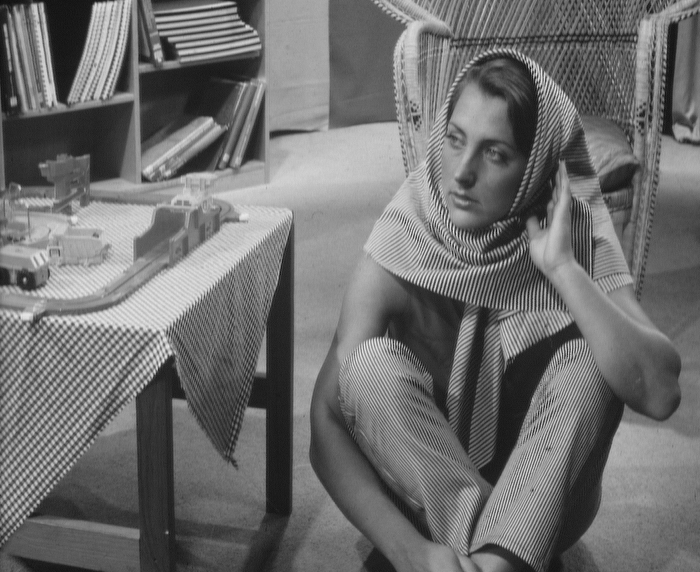
\includegraphics[width=0.8\linewidth]{f/gbarbara.png}~$u$

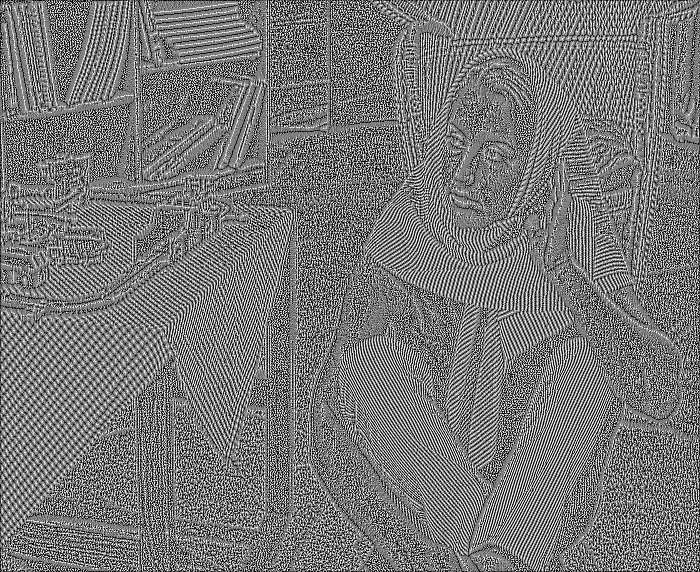
\includegraphics[width=0.8\linewidth]{f/barbara_rank1.png}~rank~$1$

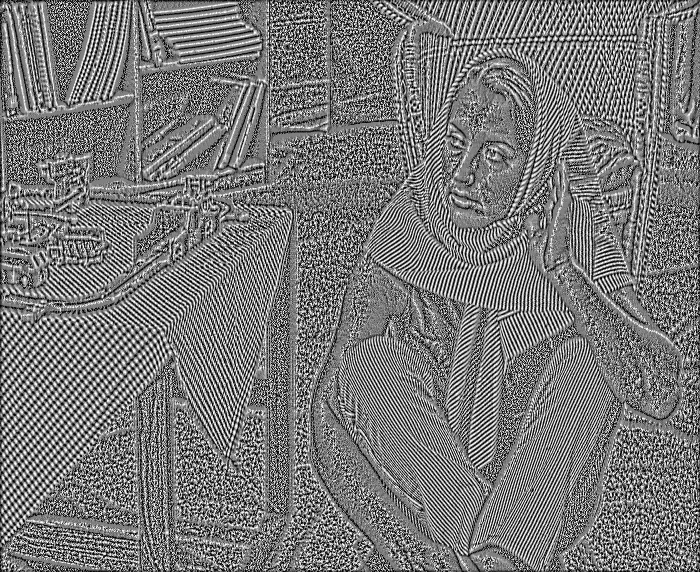
\includegraphics[width=0.8\linewidth]{f/barbara_rank3.png}~rank~$3$

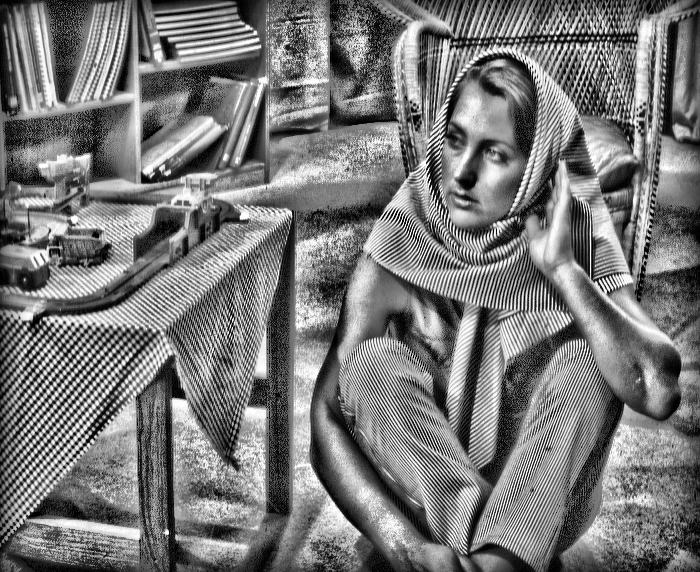
\includegraphics[width=0.8\linewidth]{f/barbara_rank30.png}~rank~$30$

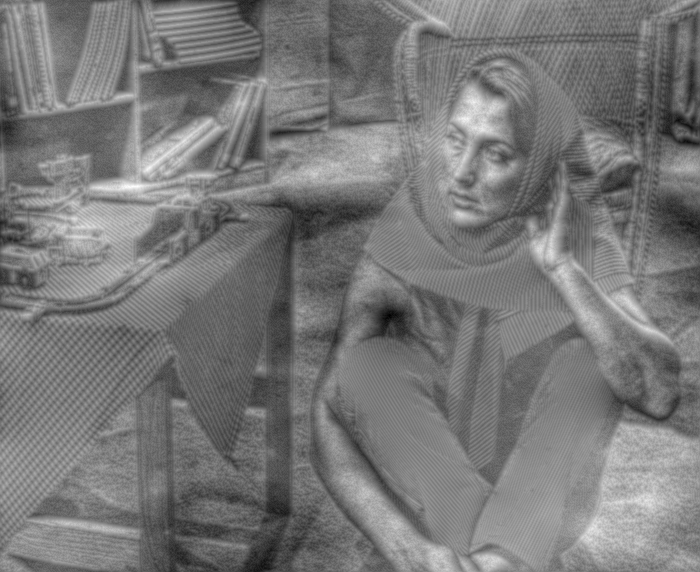
\includegraphics[width=0.8\linewidth]{f/barbara_poisnor.png}~$\Delta^{-1}
\mathrm{div}\left(\frac{\nabla u}{\left\|\nabla u\right\|}\right)$

\end{document}


% vim:set tw=76 filetype=tex spell spelllang=en:
